\section*{Methodology}

\begin{frame}
    \begin{enumerate}
        \setcounter{enumi}{1}
        \item Methodology: by Ayush Raina
    \end{enumerate}
\end{frame}

\begin{frame}{Methodology}
    \begin{block}{Distance Restraints and Energy Assisted Modelling}
        DREAM algorithm uses distance restraints obtained from NMR data to model the structure of proteins in 3 steps:
        \begin{enumerate}
            \item \textbf{Construction of Substructures:} We divide the available distance restraints data into dense fragments and model their structure first.
        \end{enumerate}
        \pause
        \begin{figure}[h]
            \centering
            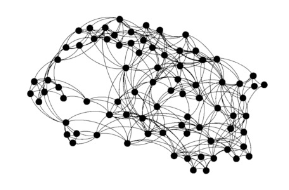
\includegraphics[width=0.35\textwidth]{images/single.png}
            \pause
            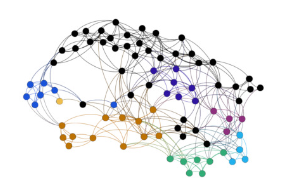
\includegraphics[width=0.35\textwidth]{images/separate.png}
            \caption{Dividing into dense fragments}
            \label{fig:my_label}
        \end{figure}
    \end{block}
\end{frame}

\begin{frame}{DREAM}
    \begin{enumerate}
        \setcounter{enumi}{1}
        \item \textbf{One Shot Registration:} We then join all the substructures into a single structure at once instead of sequential registration.
    \end{enumerate}

    \pause 

    \begin{figure}[h]
        \centering
        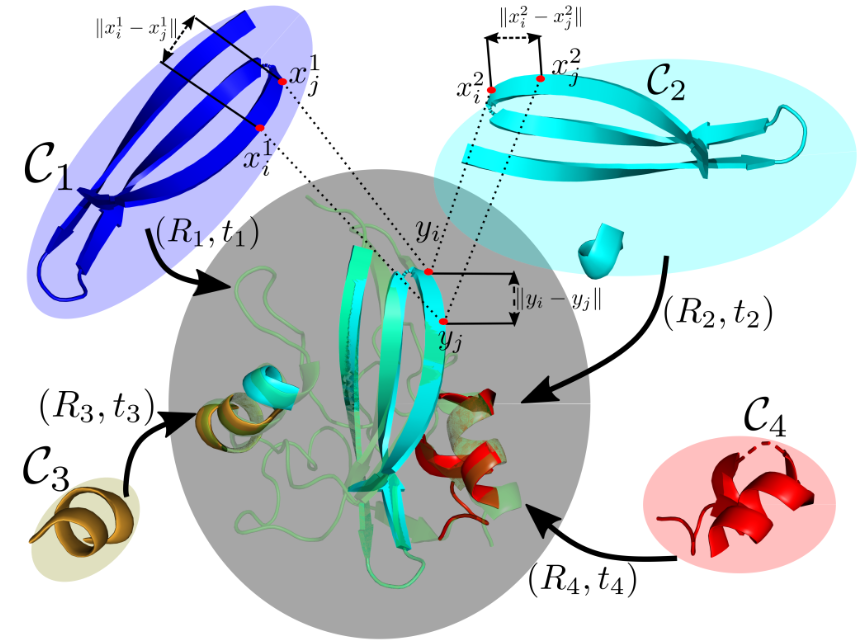
\includegraphics[width=0.45\textwidth]{images/register.png}
        \caption{One Shot Registration}
        \label{fig:my_label}
    \end{figure}

    Here $(R,t)$ denotes the rotation and translation of the substructure.
\end{frame}

\begin{frame}{DREAM}
    \begin{enumerate}
        \setcounter{enumi}{2}
        \item \textbf{Gap Filling:} Here many hybrid approaches are used to model the missing regions in the structure. This includes energy minimization, water refinement etc. 
    \end{enumerate}

    \begin{figure}[h]
        \centering
        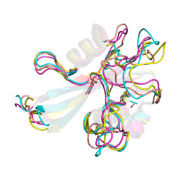
\includegraphics[width=0.4\textwidth]{images/gap1.png}
        \pause
        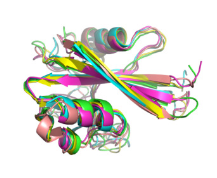
\includegraphics[width=0.4\textwidth]{images/gap2.png}
        \caption{Gap Filling}
        \label{fig:my_label}
    \end{figure}
\end{frame}

\begin{frame}{But why DREAM ?}
    \begin{itemize}
        \item Uses divide and conquer approach which increases robustness and scalability.
        \pause
        \item Reduces numerical instabilities because of the use of dense fragments.
        \pause
        \item In sequential registration, the error keeps on accumulating which is not the case in one shot registration.
    \end{itemize}
\end{frame}

\begin{frame}{Sequential vs One Shot Registration}
    \begin{figure}[h]
        \centering
        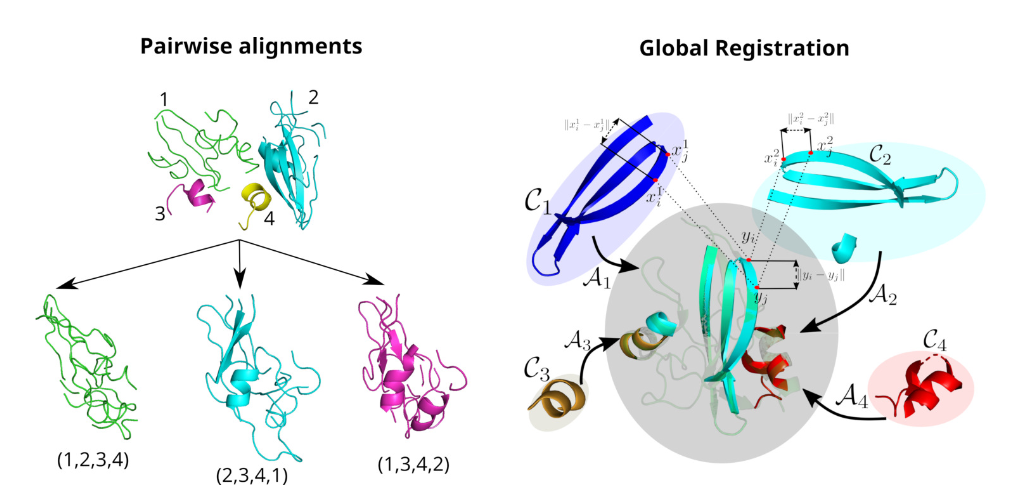
\includegraphics[width=1\textwidth]{images/seq.png}
        \caption{Sequential vs One shot registration}
        \label{fig:my_label}
    \end{figure}
\end{frame}